\section{Pratical case}
In this section, we'll comment on a practical case of the use of deepfake as a disinformation tool.
Indeed, a deployment of Russian soldiers on the Ukrainian border has heightened tensions between Russia and the West. Vladimir Putin, the Russian president, declared war on Ukraine at dawn on February 24, 2022, after having recognized the independence of the two pro-Russian separatist territories of the Ukrainian Donbass a few days earlier. Several of the country's major cities, including the capital Kiev, have been hit by bombs since the Russian army invaded. Ukrainian authorities are reporting thousands of deaths, and Russian military forces are attacking on several fronts in addition to air strikes. Evacuation of civilians is becoming increasingly difficult as many choose to resist and fight alongside the army of Ukrainian President Volodymyr Zelensky. Millions of Ukrainian refugees are trying to flee the conflict in every possible way.

In that context since the 24th of February 2022, several public and private 
media, and even individuals' personal accounts, have been relaying informations on the progress of the situation.  And it can easily become difficult to distinguish good information from bad.  On Monday June 5, 2023, several  videos were broadcast in which Vladimir Poutine  spoke on Russian television, as shown in the figure below.
\
\begin{figure}[h]
    \centering
    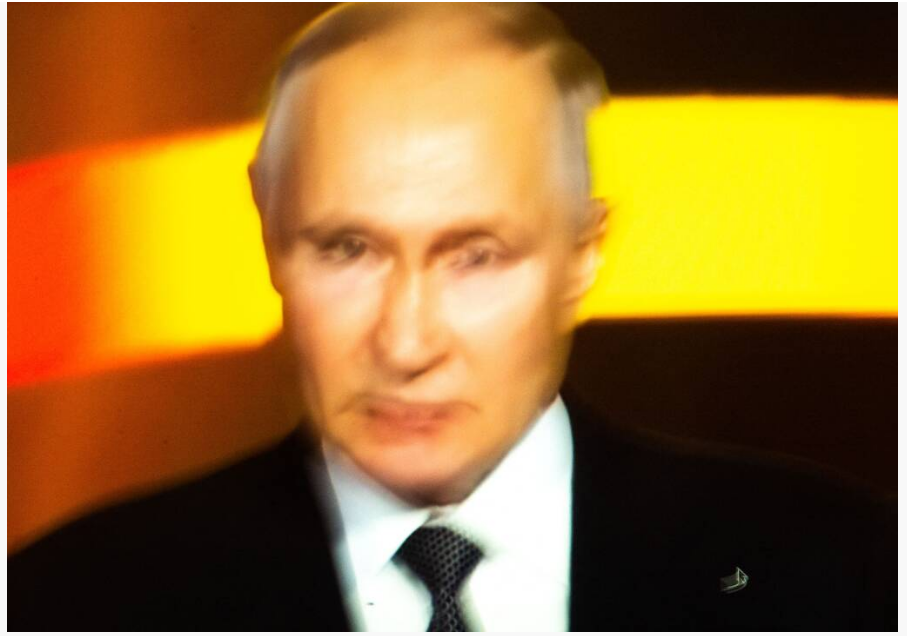
\includegraphics[width=0.5\linewidth]{images/poutine.PNG}
    \caption{Vladimir Poutine \cite{coquazDeepfakeFauxMessage}}
    \label{fig:enter-label}
\end{figure}


 \emph{In this emergency address to the nation, the Russian president would announce the arrival of Ukrainian troops in the regions of Kursk, Belgorod and Bryansk, according to the Russian-language media Holod, as well as a general mobilization and the introduction of martial law to deal with it \cite{coquazDeepfakeFauxMessage}.}
Many people believed it because of the similarity between the voice on the recording and that of the president. But Vladimir Poutine did not take the floor on Monday June 5 for an emergency address to the nation, it was all the result of deepfake disinformation. 
\emph{In this instance, the general consensus was that the Russian president's voice was particularly well imitated (although some astute Russian speakers noted subtle accent inconsistencies on certain words). Making the address potentially credible, especially in its radio version (while the video version suffers from unnatural movements of the "fake Putin's" mouth) \cite{coquazDeepfakeFauxMessage}.}
Analysis of this situation clearly shows that this deepfake has created confusion and misinformation among the population, undermining trust in the media and official discourse. In the context of this conflict, this could have aggravated tensions and further complicated diplomatic negotiations. The Russian news agency Tass, perhaps to avoid panic, quickly confirmed the incident, stating that \emph{Russian President Vladimir Putin made no emergency address on TV or radio on June 5. The video broadcast on some networks is [the result of] hacking, and experts are already dealing with it, presidential press officer Dmitry Peskov told Tass.\cite{coquazDeepfakeFauxMessage}}